\chapter{Design}

\section{Conceptual Model}

\subsection{State Diagram}
\begin{figure}[ht]
\centering
\empuse{erdiag}
\caption{Entity Relationship Diagram}
\end{figure}
\FloatBarrier

\subsection{Activity Diagrams}

\begin{figure}[ht]
\centering
\empuse{activityR1}
\caption{Activity Diagram: Creating a project.}
\end{figure}


\begin{figure}[ht]
\centering
\empuse{activityR2}
\caption{Activity Diagram: Creating a team.}
\end{figure}


\begin{figure}[ht]
\centering
\empuse{activityR4}
\caption{Activity Diagram: Assigning tasks.}
\end{figure}
\FloatBarrier

\subsection{Mockups}

\begin{figure}[ht]
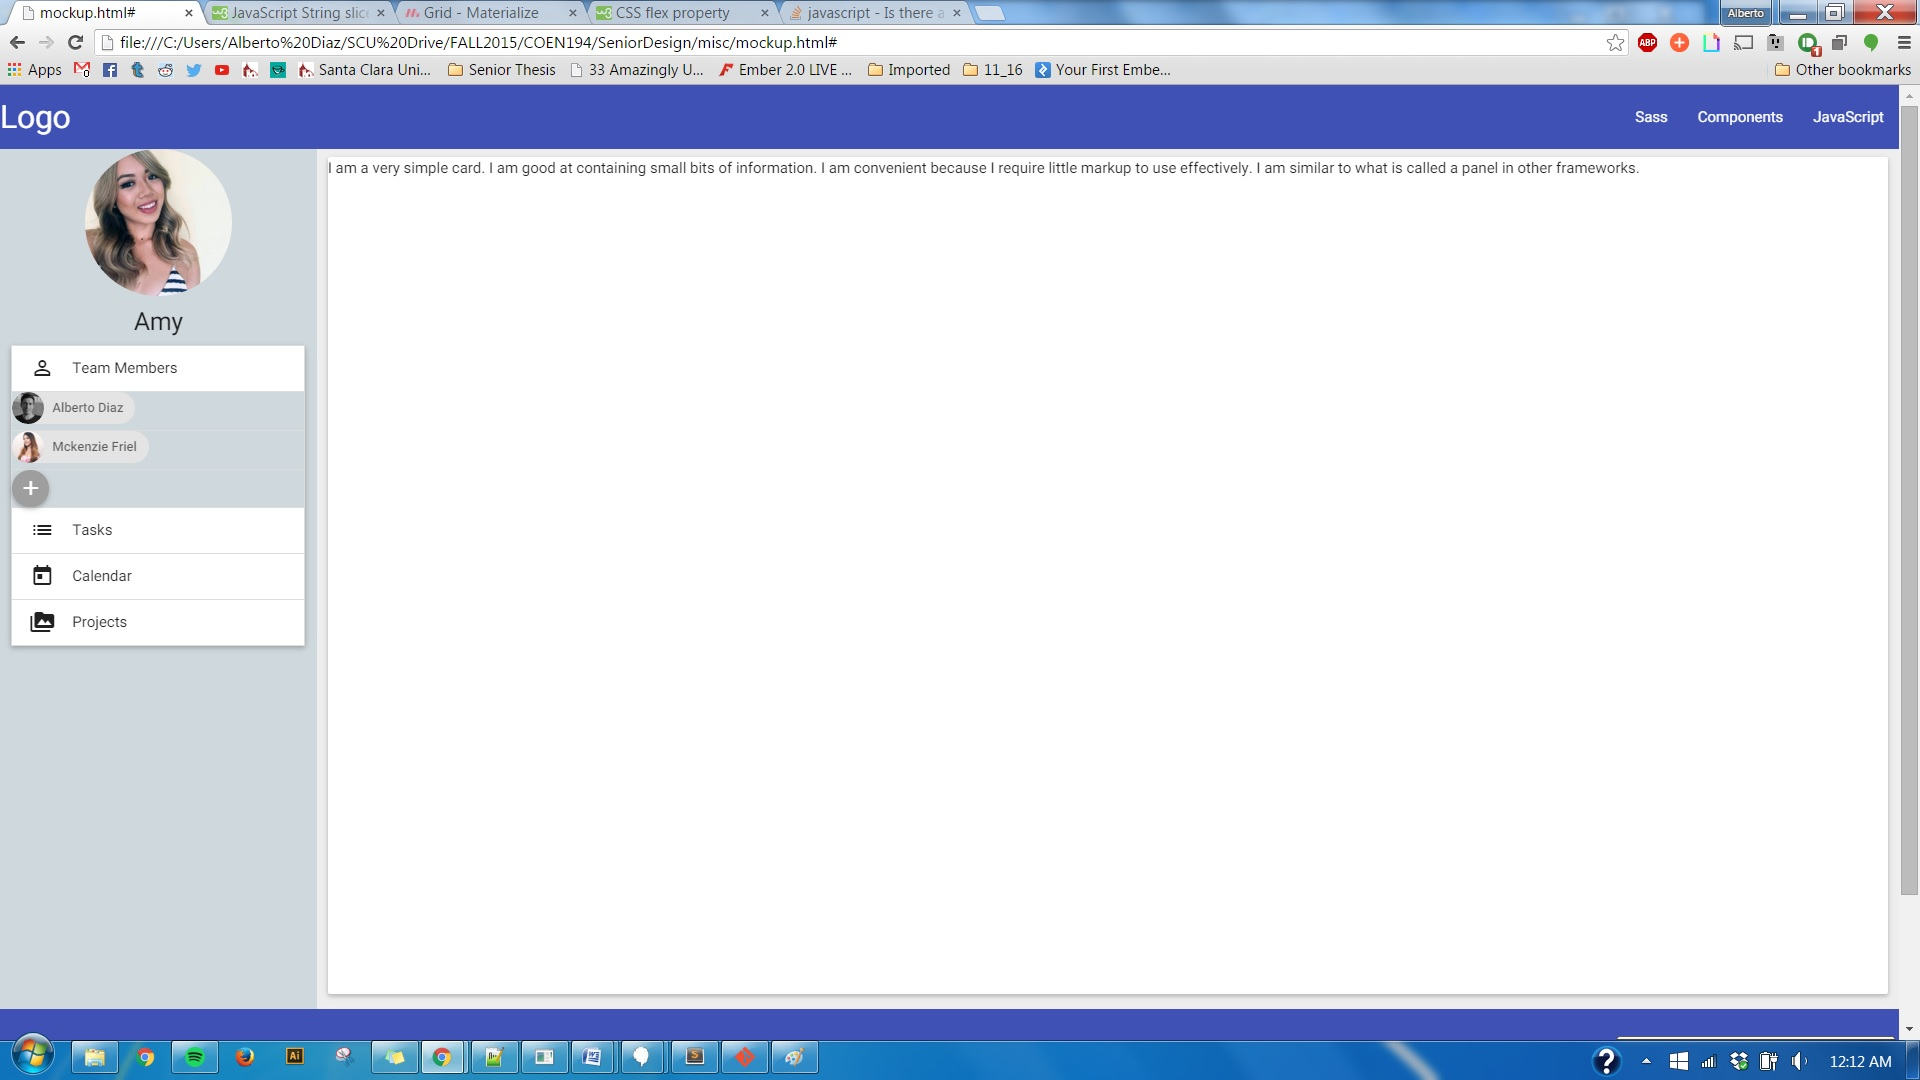
\includegraphics[width=\textwidth]{mockup.jpg}
\caption{A mockup of our system concept.}
\end{figure}
\FloatBarrier

\section{Use Cases}
A use case defines the steps required to accomplish a specific goal. The following use cases describe how the user interacts with the system to achieve these goals, including preconditions, postconditions, steps required, and common errors that might occur. The use case diagram, Figure XXX, helps to illustrate the user’s major actions in our application: creating a project, adding team members, and creating and assigning tasks. 
\begin{figure}[ht]
\centering
\empuse{usecasediag}
\caption{Use Case Diagram}
\end{figure}

\begin{figure}[ht]
\begin{usecase}

\addtitle{Use Case 1}{Create Project} 

\addfield{Goal:}{Initialize project objectives, tasks, and deadlines}

\addfield{Actor:}{User}

\addfield{Preconditions:}{Account is set up and logged in}
%when multiple
%\additemizedfield{Preconditions:}{} 

\addfield{Postconditions:}{Project is initialized}
%when multiple
%\additemizedfield{Preconditions:}{}

%Main Success Scenario: A typical, unconditional happy path scenario of success.
\addscenario{Steps:}{
  \item Name the project
  \item Define project goals and deadlines
  \item Add people to the project
  \item Save the project
}

%Extensions: Alternate scenarios of success or failure.
\addscenario{Exceptions:}{
  \item[A.] Invalid login data:
    \begin{enumerate}
    \item[1.] System shows failure message
    \item[2.] User returns to step 1
    \end{enumerate}
}
\end{usecase}
\end{figure}
\begin{figure}[ht]
\begin{usecase}

\addtitle{Use Case 2}{Add team members} 

\addfield{Goal:}{Associate people with the project}

\addfield{Actor:}{User}

\addfield{Preconditions:}{Logged in, project created}
%when multiple
%\additemizedfield{Preconditions:}{} 

\addfield{Postconditions:}{Project has people assigned}
%when multiple
%\additemizedfield{Preconditions:}{}

%Main Success Scenario: A typical, unconditional happy path scenario of success.
\addscenario{Steps:}{
  \item Enter team description
  \item Enter member contact
  \item If found, add member 
}

%Extensions: Alternate scenarios of success or failure.
\addscenario{Exceptions:}{
  \item[2.a] Invalid login data:
    \begin{enumerate}
    \item[1.] System shows failure message
    \item[2.] User returns to step 1
    \end{enumerate}
  \item[5.a] Invalid subsriber data:
    \begin{enumerate}
    \item[1.] System shows failure message
    \item[2.] User returns to step 2 and corrects the errors
    \end{enumerate}
}
\end{usecase}
\end{figure}
\begin{figure}[ht]
\begin{usecase}

\addtitle{Use Case 1}{Template test} 

\addfield{Goal:}{System-wide}

\addfield{Actor:}{End-User}

\addfield{Preconditions:}{}
%when multiple
%\additemizedfield{Preconditions:}{} 

\addfield{Postconditions:}{}
%when multiple
%\additemizedfield{Preconditions:}{}

%Main Success Scenario: A typical, unconditional happy path scenario of success.
\addscenario{Steps:}{
  \item The first action
  \item The second action
}

%Extensions: Alternate scenarios of success or failure.
\addscenario{Exceptions:}{
  \item[2.a] Invalid login data:
    \begin{enumerate}
    \item[1.] System shows failure message
    \item[2.] User returns to step 1
    \end{enumerate}
  \item[5.a] Invalid subsriber data:
    \begin{enumerate}
    \item[1.] System shows failure message
    \item[2.] User returns to step 2 and corrects the errors
    \end{enumerate}
}
\end{usecase}
\end{figure}
\FloatBarrier

\section{Architectural Design}
\begin{figure}[ht]
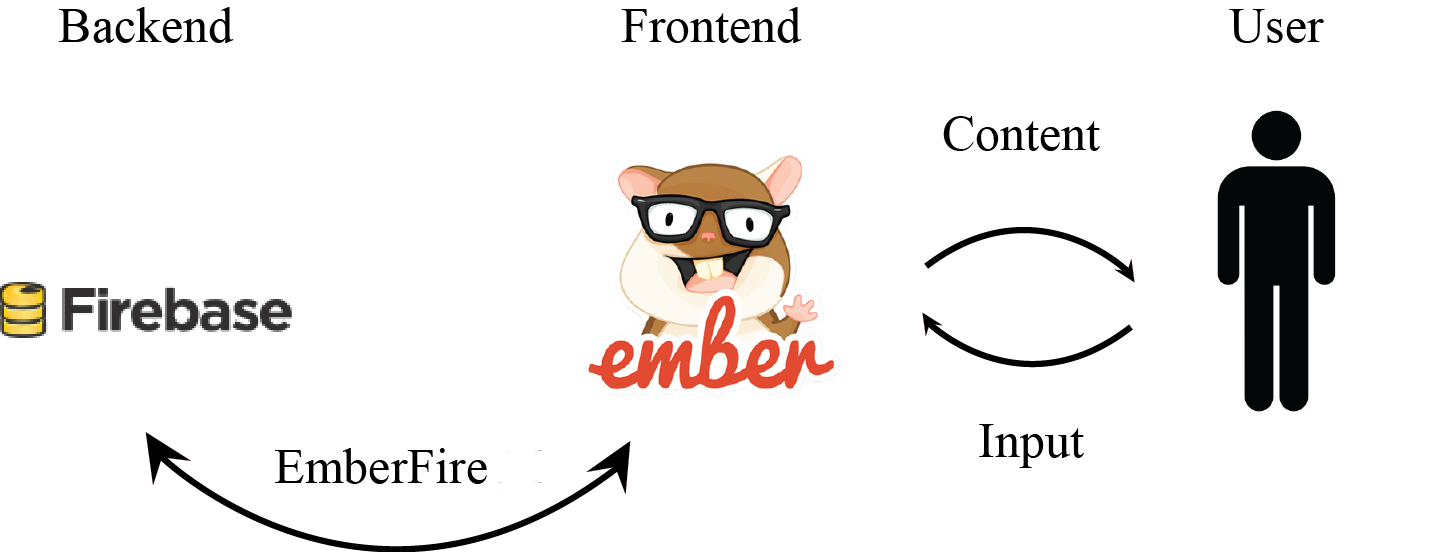
\includegraphics[width=\textwidth]{archDiag.png}
\caption{Diagram describing the technology stack for our application.}
\end{figure}
\FloatBarrier

\section{Technologies Used}
In this section, we describe the technologies we chose to develop our application and the features they provide for us.
\begin{enumerate}
\item HTML5 \par The latest version of the standard web markup language
\item JS \par A high-level, untyped, and interpreted programming  language supported by all modern web browser
\item CSS3 \par A stylesheet language used to describe the presentation of HTML documents
\item Ember.js \par A front-end javascript framework based on the model-view-controller (MVC) model and applies programming conventions to build scalable applications
\item  Firebase \par A backend-as-a-service that provides client-side APIs, and services such as databases, web hosting, and authentication.
\end{enumerate}

\section{Design Rationale}
In this section, we describe why we chose these technologies and the advantages and disadvantages associated with each of those technologies. 
\begin{enumerate}
\item HTML5/CSS3 /JS \par This trio of web technologies has become the standard for web development
	\begin{enumerate}
		\item Advantages
		\begin{enumerate}
			\item Well documented and supported in the development community
			\item Gives the developer control over the look and feel of the application
			\item Compatible with nearly any web browser out there
		\end{enumerate}
		\item Disadvantages
		\begin{enumerate}
			\item Without a framework or library it has little functionality
			\item Requires a lot of time and effort to create a complete and robust application
			\item Some browser interpret certain elements differently
		\end{enumerate}
	\end{enumerate}
\item Ember.js \par We chose a framework because it expedites the development process. Ember.js boasts taking its developers 80\% of the way through development with the use of best idioms and proper practices. It is used by companies such as Yahoo, Groupon, and Square.
	\begin{enumerate}
		\item Advantages
		\begin{enumerate}
			\item Faster development start time
			\item Allows the developer to create reusable components through the use Handlebars templates
			\item The built in router allows developers to create multi page applications by navigating the user through states rather than physical webpages, reducing the need to keep track of these different states since the page never physically reloads. 
		\end{enumerate}
		\item Disadvantages
		\begin{enumerate}
			\item The framework is based around conventions, limiting developers freedom for a majority of the development process
			\item If the developers do stray from convention, they could find themselves having a difficult time reaching completion
		\end{enumerate}
	\end{enumerate}
\item  Firebase \par We chose this backend service due to the fact that it provides a client-side API for Ember.js called EmberFire.
	\begin{enumerate}
		\item Advantages
		\begin{enumerate}
			\item Using a client-side API eliminates the need for a backend language and allow us to focus on a single language for all of our development.
			\item Firebase also provides hosting and database services for free!
		\end{enumerate}
		\item Disadvantages
		\begin{enumerate}
			\item Support is outsourced, we do not have direct access to our server and are at the mercy of whatever functionality is provided by the API
			\item A free firebase account does not provide provide private backups of our data, increasing the probability of data loss
		\end{enumerate}
	\end{enumerate}
\end{enumerate}